\chapter{Diseño de datos} \label{cap:diseño_datos}

\section{Introducción}
En este capítulo se definirán las estructuras de datos que conforman el sistema a partir de los elementos identificados durante el análisis de datos del Capítulo 7 (tipos de entidad y tipos de interrelación). Para ello, se llevarán a cabo los siguientes pasos:

\begin{itemize}
    \item Obtención del modelo relacional. Definición de la estructuras (tablas) del modelo de datos.
    \item Normalización del modelo. Refinamiento del modelo, para la eliminación de errores de integridad.
    \item Obtención del esquema relacional.
    \item Diagrama relacional.
\end{itemize}

 \section{Modelo Relacional}\label{sec:modelo-relacional}
A partir del Modelo Entidad - Interrelación descrito en el capítulo 7, se pueden obtener las tablas o relaciones del Modelo Relacional utilizando las reglas de transformación (RTECAR - véase el capítulo 5 de Bases de Datos. Desde Chen hasta Codd con ORACLE.\cite{reglasBD}). En concreto, se han aplicado las siguientes reglas de transformación:

\begin{itemize}
    \item RTECAR-1: Todos los tipos de entidad presentes en el esquema conceptual se transformarán en tablas o relaciones en el esquema relacional manteniendo el número y tipo de atributos, así como la característica de identificador de esos atributos.
    \item RTECAR-3.1: En las relaciones 1:N, la clave primaria de la entidad del lado 1 se convierte en una clave foránea en la tabla de la entidad del lado N.
\end{itemize}

Para cada tabla se mostrará la siguiente información:

\begin{itemize}
    \item \textbf{Descripción}. Se describirá el origen de la tabla, indicando los elementos del modelo Entidad-Interrelación desde los que se ha obtenido.
    \item \textbf{Nombre de la tabla}
    \item \textbf{Atributos}. Se describirán los atributos que componen la tabla, distinguiendo su rol en cada caso con la siguiente notación:
        \begin{itemize}
            \item Clave \underline{primaria}
            \item Clave ALTERNA, si existe
            \item Claves \textbf{foráneas}, si existen
            \item Resto de atributos
        \end{itemize}
    \item \textbf{Esquema relacional}. Definición formal de la tabla, de acuerdo con el Modelo Relacional.
\end{itemize}

\subsection{Tabla Tipo Centro}
    \begin{itemize}
        \item \textbf{Descripción}: la tabla Tipo Centro se obtiene a partir de la entidad \textit{Tipo Centro}.
        \item \textbf{Nombre de la tabla}: TipoCentro
        \item \textbf{Atributos}:
            \begin{itemize}
                \item Clave primaria: \underline{id}
                \item Clave alterna: ninguna.
                \item Clave foránea: ninguna.
                \item Resto de atributos: nombre, estado.
            \end{itemize}
        \item \textbf{Esquema relacional}: 
            TipoCentro (\textbf{\underline{id}}, nombre, estado)
    \end{itemize}

\subsection{Tabla Tipo Representación Gobierno}
    \begin{itemize}
        \item \textbf{Descripción}: la tabla Tipo Representación Gobierno se obtiene a partir de la entidad \textit{Tipo Representación Gobierno}.
        \item \textbf{Nombre de la tabla}: TipoRepresentaciónGobierno
        \item \textbf{Atributos}:
            \begin{itemize}
                \item Clave primaria: \underline{id}
                \item Clave alterna: ninguna
                \item Clave foránea: ninguna
                \item Resto de atributos: nombre, estado.
            \end{itemize}
        \item \textbf{Esquema relacional}: 
            TipoRepresentaciónGobierno(\textbf{\underline{id}}, nombre, estado)
    \end{itemize}

\subsection{Tabla Tipo Representación General}
    \begin{itemize}
        \item \textbf{Descripción}: la tabla Tipo Representación General se obtiene a partir de la entidad \textit{Tipo Representación General}.
        \item \textbf{Nombre de la tabla}: TipoRepresentaciónGeneral
        \item \textbf{Atributos}:
            \begin{itemize}
                \item Clave primaria: \underline{id}
                \item Clave alterna: ninguna
                \item Clave foránea: ninguna
                \item Resto de atributos: nombre, estado.
            \end{itemize}
        \item \textbf{Esquema relacional}: 
            TipoRepresentaciónGeneral(\textbf{\underline{id}}, nombre, estado)
    \end{itemize}

\subsection{Tabla Tipo Convocatoria}
    \begin{itemize}
        \item \textbf{Descripción}: la tabla Tipo Convocatoria se obtiene a partir de la entidad \textit{Tipo Convocatoria}.
        \item \textbf{Nombre de la tabla}: TipoRepresentaciónGeneral
        \item \textbf{Atributos}:
            \begin{itemize}
                \item Clave primaria: \underline{id}
                \item Clave alterna: ninguna
                \item Clave foránea: ninguna
                \item Resto de atributos: nombre, estado.
            \end{itemize}
        \item \textbf{Esquema relacional}: 
            TipoConvocatoria(\textbf{\underline{id}}, nombre, estado)
    \end{itemize}

\subsection{Tabla Usuario}
    \begin{itemize}
        \item \textbf{Descripción}: la tabla Usuario se obtiene a partir de la entidad \textit{Usuario}.
        \item \textbf{Nombre de la tabla}:
        \item \textbf{Atributos}:
            \begin{itemize}
                \item Clave primaria: \underline{id}
                \item Clave alterna: 
                \item Clave foránea: \textbf{}
                \item Resto de atributos: 
            \end{itemize}
        \item \textbf{Esquema relacional}: 
            Usuario(\textbf{\underline{id}}, name, email, password, estado)
    \end{itemize}

\subsection{Tabla Centro}
    \begin{itemize}
        \item \textbf{Descripción}: la tabla Centro se obtiene a partir de la entidad \textit{Centro}. Además, se incorpora la clave foránea \textbf{idTipo} de la tabla TipoCentro porque el tipo de entidad Centro presenta una debilidad por identificación respecto del tipo de entidad Tipo Centro.
        \item \textbf{Nombre de la tabla}: Centro
        \item \textbf{Atributos}:
            \begin{itemize}
                \item Clave primaria: \underline{id}
                \item Clave alterna: ninguna
                \item Clave foránea: \textbf{idTipo}
                \item Resto de atributos: nombre, dirección, estado
            \end{itemize}
        \item \textbf{Esquema relacional}: 
            Centro(\textbf{\underline{id}}, nombre, dirección, idTipo, estado)
    \end{itemize}

\subsection{Tabla Junta}
    \begin{itemize}
        \item \textbf{Descripción}: la tabla Junta se obtiene a partir de la entidad \textit{Junta}. Además, se incorpora la clave foránea \textbf{idCentro} de la tabla Centro porque el tipo de entidad Junta presenta una debilidad por identificación respecto del tipo de entidad Centro.
        \item \textbf{Nombre de la tabla}: Junta
        \item \textbf{Atributos}:
            \begin{itemize}
                \item Clave primaria: \underline{id}
                \item Clave alterna: ninguna
                \item Clave foránea: \textbf{idCentro}
                \item Resto de atributos: fechaConstitución, fechaDisolución, estado
            \end{itemize}
        \item \textbf{Esquema relacional}: 
            Junta(\textbf{\underline{id}}, fechaConstitución, fechaDisolución, idCentro, estado)
    \end{itemize}

\subsection{Tabla Comisión}
    \begin{itemize}
        \item \textbf{Descripción}: la tabla Comisión se obtiene a partir de la entidad \textit{Comisión}. Además, se incorpora la clave foránea \textbf{idJunta} de la tabla Junta porque el tipo de entidad Comisión presenta una debilidad por identificación respecto del tipo de entidad Junta.
        \item \textbf{Nombre de la tabla}: Comisión
        \item \textbf{Atributos}:
            \begin{itemize}
                \item Clave primaria: \underline{id}
                \item Clave alterna: ninguna
                \item Clave foránea: \textbf{idJunta}
                \item Resto de atributos: nombre, descripción, fechaConstitución, fechaDisolución, estado
            \end{itemize}
        \item \textbf{Esquema relacional}: 
            Comisión(\textbf{\underline{id}}, nombre, descripción, fechaConstitución, fechaDisolución, idJunta, estado)
    \end{itemize}

\subsection{Tabla Convocatoria}
    \begin{itemize}
        \item \textbf{Descripción}: la tabla Convocatoria se obtiene a partir de la entidad \textit{Convocatoria}. Además, se incorpora la clave foránea \textbf{idJunta} de la tabla Junta porque el tipo de entidad Convocatoria presenta una debilidad por identificación respecto del tipo de entidad Junta. Se incorpora la clave foránea \textbf{idComisión} de la tabla Comisión porque el tipo de entidad Convocatoria presenta una debilidad por identificación respecto del tipo de entidad Comisión. Se incorpora la clave foránea \textbf{idTipo} de la tabla TipoConvocatoria porque el tipo de entidad Convocatoria presenta una debilidad por identificación respecto del tipo de entidad TipoConvocatoria.
        \item \textbf{Nombre de la tabla}: Convocatoria
        \item \textbf{Atributos}:
            \begin{itemize}
                \item Clave primaria: \underline{id}
                \item Clave alterna: ninguna
                \item Clave foránea: \textbf{idJun}, \textbf{idCom}, \textbf{idTipo}
                \item Resto de atributos: lugar, fecha, hora, estado
            \end{itemize}
        \item \textbf{Esquema relacional}: 
            Convocatoria(\textbf{\underline{id}}, lugar, fecha, hora, idTipo, idJun, idCom, estado)
    \end{itemize}

\subsection{Tabla Miembro Gobierno}
    \begin{itemize}
        \item \textbf{Descripción}: la tabla MiembroGobierno se obtiene a partir de la entidad \textit{Miembro Gobierno}. Además, se incorpora la clave foránea \textbf{idUsuario} de la tabla Junta porque el tipo de entidad MiembroGobierno presenta una debilidad por identificación respecto del tipo de entidad Usuario. Se incorpora la clave foránea \textbf{idCentro} de la tabla Centro porque el tipo de entidad MiembroGobierno presenta una debilidad por identificación respecto del tipo de entidad Centro. Se incorpora la clave foránea \textbf{idRepresentación} de la tabla TipoRepresentaciónGobierno porque el tipo de entidad MiembroGobierno presenta una debilidad por identificación respecto del tipo de entidad TipoRepresentaciónGobierno.
        \item \textbf{Nombre de la tabla}: MiembroGobierno
        \item \textbf{Atributos}:
            \begin{itemize}
                \item Clave primaria: \underline{id}
                \item Clave alterna: ninguna
                \item Clave foránea: \textbf{idUsuario}, \textbf{idCentro}, \textbf{idRepresentación}
                \item Resto de atributos: fechaTomaPosesión, fechaCese, estado
            \end{itemize}
        \item \textbf{Esquema relacional}: 
            MiembroGobierno(\textbf{\underline{id}}, fechaTomaPosesión, fechaCese, idUsuario, idCentro, idRepresentación, estado)
    \end{itemize}

\subsection{Tabla Miembro Junta}
    \begin{itemize}
        \item \textbf{Descripción}: la tabla MiembroJunta se obtiene a partir de la entidad \textit{Miembro Junta}. Además, se incorpora la clave foránea \textbf{idUsuario} de la tabla Junta porque el tipo de entidad MiembroJunta presenta una debilidad por identificación respecto del tipo de entidad Usuario. Se incorpora la clave foránea \textbf{idJunta} de la tabla Centro porque el tipo de entidad MiembroJunta presenta una debilidad por identificación respecto del tipo de entidad Junta. Se incorpora la clave foránea \textbf{idRepresentación} de la tabla TipoRepresentaciónGeneral porque el tipo de entidad MiembroJunta presenta una debilidad por identificación respecto del tipo de entidad TipoRepresentaciónGeneral.
        \item \textbf{Nombre de la tabla}: MiembroGobierno
        \item \textbf{Atributos}:
            \begin{itemize}
                \item Clave primaria: \underline{id}
                \item Clave alterna: ninguna
                \item Clave foránea: \textbf{idUsuario}, \textbf{idJunta}, \textbf{idRepresentación}
                \item Resto de atributos: fechaTomaPosesión, fechaCese, estado
            \end{itemize}
        \item \textbf{Esquema relacional}: 
            MiembroJunta(\textbf{\underline{id}}, fechaTomaPosesión, fechaCese, idUsuario, idJunta, idRepresentación, estado)
    \end{itemize}

\subsection{Tabla Miembro Comisión}
    \begin{itemize}
        \item \textbf{Descripción}: la tabla MiembroComisión se obtiene a partir de la entidad \textit{Miembro Comisión}. Además, se incorpora la clave foránea \textbf{idUsuario} de la tabla Junta porque el tipo de entidad MiembroComisión presenta una debilidad por identificación respecto del tipo de entidad Usuario. Se incorpora la clave foránea \textbf{idComisión} de la tabla Centro porque el tipo de entidad MiembroJunta presenta una debilidad por identificación respecto del tipo de entidad Comisión. Se incorpora la clave foránea \textbf{idRepresentación} de la tabla TipoRepresentaciónGeneral porque el tipo de entidad MiembroJunta presenta una debilidad por identificación respecto del tipo de entidad TipoRepresentaciónGeneral.
        \item \textbf{Nombre de la tabla}: MiembroComisión
        \item \textbf{Atributos}:
            \begin{itemize}
                \item Clave primaria: \underline{id}
                \item Clave alterna: ninguna
                \item Clave foránea: \textbf{idUsuario}, \textbf{idComisión}, \textbf{idRepresentación}
                \item Resto de atributos: fechaTomaPosesión, fechaCese, estado
            \end{itemize}
        \item \textbf{Esquema relacional}: 
            MiembroComisión(\textbf{\underline{id}}, fechaTomaPosesión, fechaCese, idUsuario, idComisión, idRepresentación, estado)
    \end{itemize}
    
 \section{Normalización del modelo}\label{sec:normalizacion}
La normalización del modelo descrito en la sección anterior pretende detectar y corregir redundancias e inconsistencias en la información representada, para lo cual se aplicarán las medidas correctoras que garanticen que las tablas obtenidas cumplen las siguientes formas normalizadas \cite{reglasBD}.

\begin{itemize}
    \item Primera Forma Normal (FN1): una relación R satisface la FN1 si y solo si, todos los dominios subyacentes de la relación R (atributos) contienen valores atómicos.
    \item Segunda Forma Normal (FN2): una relación R satisface la FN2 si y sólo si, satisface la FN1 y cada atributo de la relación depende funcionalmente de forma completa de la clave primaria de esa relación.
    \item Tercera Forma Normal (FN3): una relación R satisface la FN3 si y sólo si, satisface la FN2 y cada atributo no primo de la relación no depende funcionalmente de forma transitiva de la clave primaria de esa relación, es decir, no pueden existir dependencias transitivas entre los atributos que no forman parte de la clave primaria de esa relación R.
    \item Forma Normal de Boyce-Codd (FNBC): una relación R satisface la FNBC si y sólo si, se encuentra en FN1 y cada determinante funcional es una clave candidata de la relación R, denominándose determinante funcional a uno o un conjunto de atributos de una relación R del cual depende funcionalmente de forma completa algún otro atributo de la misma relación.
\end{itemize}

Todas las tablas definidas se encuentran en la Primera Forma Normal, puesto que en ninguna de ellas existen atributos múltiples.

\subsection{Tabla TipoCentro}
    \begin{itemize}
        \item \textbf{Claves candidatas}: id
        \item \textbf{Normalización}: La tabla TipoCentro presenta una dependencia funcional formada por la clave primaria y el resto de atributos. La tabla se encuentra en FNBC: el único determinante funcional es la clave primaria, por lo que la dependencia funcional con el resto de atributos es completa.
    \end{itemize}

\begin{figure}[H]
\centering
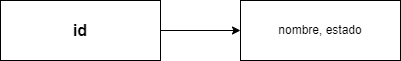
\includegraphics[scale=0.75]{img/diagramas/Datos/FNBC-TipoCentro.png}
\caption{Tabla TipoCentro en FNBC}\label{fig:Tabla TipoCentro en FNBC}   
\end{figure}

\subsection{Tabla TipoRepresentaciónGobierno}
    \begin{itemize}
        \item \textbf{Claves candidatas}: id
        \item \textbf{Normalización}: La tabla TipoRepresentaciónGobierno presenta una dependencia funcional formada por la clave primaria y el resto de atributos. La tabla se encuentra en FNBC: el único determinante funcional es la clave primaria, por lo que la dependencia funcional con el resto de atributos es completa.
    \end{itemize}

\begin{figure}[H]
\centering
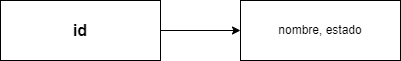
\includegraphics[scale=0.75]{img/diagramas/Datos/FNBC-TipoRepresentaciónGobierno.png}
\caption{Tabla TipoRepresentaciónGobierno en FNBC}\label{fig:Tabla TipoRepresentaciónGobierno en FNBC}   
\end{figure}

\subsection{Tabla TipoRepresentaciónGeneral}
    \begin{itemize}
        \item \textbf{Claves candidatas}: id
        \item \textbf{Normalización}: La tabla TipoRepresentaciónGeneral presenta una dependencia funcional formada por la clave primaria y el resto de atributos. La tabla se encuentra en FNBC: el único determinante funcional es la clave primaria, por lo que la dependencia funcional con el resto de atributos es completa.
    \end{itemize}

\begin{figure}[H]
\centering
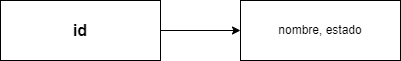
\includegraphics[scale=0.75]{img/diagramas/Datos/FNBC-TipoRepresentaciónGeneral.png}
\caption{Tabla TipoRepresentaciónGeneral en FNBC}\label{fig:Tabla TipoRepresentaciónGeneral en FNBC}   
\end{figure}

\subsection{Tabla TipoConvocatoria}
    \begin{itemize}
        \item \textbf{Claves candidatas}: id
        \item \textbf{Normalización}: La tabla TipoConvocatoria presenta una dependencia funcional formada por la clave primaria y el resto de atributos. La tabla se encuentra en FNBC: el único determinante funcional es la clave primaria, por lo que la dependencia funcional con el resto de atributos es completa.
    \end{itemize}

\begin{figure}[H]
\centering
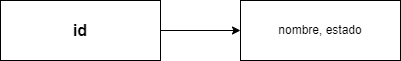
\includegraphics[scale=0.75]{img/diagramas/Datos/FNBC-TipoConvocatoria.png}
\caption{Tabla TipoConvocatoria en FNBC}\label{fig:Tabla TipoConvocatoria en FNBC}   
\end{figure}

\subsection{Tabla Usuario}
    \begin{itemize}
        \item \textbf{Claves candidatas}: id
        \item \textbf{Normalización}: La tabla Usuario presenta una dependencia funcional formada por la clave primaria y el resto de atributos. La tabla se encuentra en FNBC: el único determinante funcional es la clave primaria, por lo que la dependencia funcional con el resto de atributos es completa.
    \end{itemize}

\begin{figure}[H]
\centering
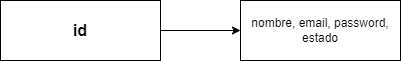
\includegraphics[scale=0.75]{img/diagramas/Datos/FNBC-Usuario.png}
\caption{Tabla Usuario en FNBC}\label{fig:Tabla Usuario en FNBC}   
\end{figure}

\subsection{Tabla Centro}
    \begin{itemize}
        \item \textbf{Claves candidatas}: id
        \item \textbf{Normalización}: La tabla Centro presenta una dependencia funcional formada por la clave primaria y el resto de atributos. La tabla se encuentra en FNBC: el único determinante funcional es la clave primaria, por lo que la dependencia funcional con el resto de atributos es completa.
    \end{itemize}

\begin{figure}[H]
\centering
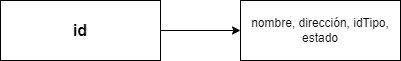
\includegraphics[scale=0.75]{img/diagramas/Datos/FNBC-Centro.png}
\caption{Tabla Centro en FNBC}\label{fig:Tabla Centro en FNBC}   
\end{figure}

\subsection{Tabla Junta}
    \begin{itemize}
        \item \textbf{Claves candidatas}: id
        \item \textbf{Normalización}: La tabla Junta presenta una dependencia funcional formada por la clave primaria y el resto de atributos. La tabla se encuentra en FNBC: el único determinante funcional es la clave primaria, por lo que la dependencia funcional con el resto de atributos es completa.
    \end{itemize}

\begin{figure}[H]
\centering
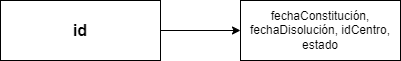
\includegraphics[scale=0.75]{img/diagramas/Datos/FNBC-Junta.png}
\caption{Tabla Junta en FNBC}\label{fig:Tabla Junta en FNBC}   
\end{figure}

\subsection{Tabla Comisión}
    \begin{itemize}
        \item \textbf{Claves candidatas}: id
        \item \textbf{Normalización}: La tabla Comisión presenta una dependencia funcional formada por la clave primaria y el resto de atributos. La tabla se encuentra en FNBC: el único determinante funcional es la clave primaria, por lo que la dependencia funcional con el resto de atributos es completa.
    \end{itemize}

\begin{figure}[H]
\centering
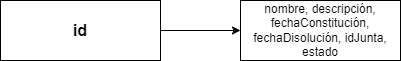
\includegraphics[scale=0.75]{img/diagramas/Datos/FNBC-Comisión.png}
\caption{Tabla Comisión en FNBC}\label{fig:Tabla Comisión en FNBC}   
\end{figure}

\subsection{Tabla Convocatoria}
    \begin{itemize}
        \item \textbf{Claves candidatas}: id
        \item \textbf{Normalización}: La tabla Convocatoria presenta una dependencia funcional formada por la clave primaria y el resto de atributos. La tabla se encuentra en FNBC: el único determinante funcional es la clave primaria, por lo que la dependencia funcional con el resto de atributos es completa.
    \end{itemize}

\begin{figure}[H]
\centering
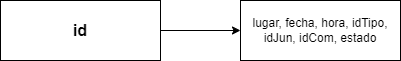
\includegraphics[scale=0.75]{img/diagramas/Datos/FNBC-Convocatoria.png}
\caption{Tabla Convocatoria en FNBC}\label{fig:Tabla Convocatoria en FNBC}   
\end{figure}

\subsection{Tabla MiembroGobierno}
    \begin{itemize}
        \item \textbf{Claves candidatas}: id
        \item \textbf{Normalización}: La tabla MiembroGobierno presenta una dependencia funcional formada por la clave primaria y el resto de atributos. La tabla se encuentra en FNBC: el único determinante funcional es la clave primaria, por lo que la dependencia funcional con el resto de atributos es completa.
    \end{itemize}

\begin{figure}[H]
\centering
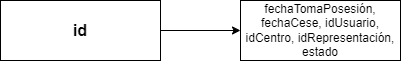
\includegraphics[scale=0.75]{img/diagramas/Datos/FNBC-MiembroGobierno.png}
\caption{Tabla MiembroGobierno en FNBC}\label{fig:Tabla MiembroGobierno en FNBC}   
\end{figure}

\subsection{Tabla MiembroJunta}
    \begin{itemize}
        \item \textbf{Claves candidatas}: id
        \item \textbf{Normalización}: La tabla MiembroJunta presenta una dependencia funcional formada por la clave primaria y el resto de atributos. La tabla se encuentra en FNBC: el único determinante funcional es la clave primaria, por lo que la dependencia funcional con el resto de atributos es completa.
    \end{itemize}

\begin{figure}[H]
\centering
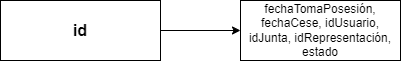
\includegraphics[scale=0.75]{img/diagramas/Datos/FNBC-MiembroJunta.png}
\caption{Tabla MiembroJunta en FNBC}\label{fig:Tabla MiembroJunta en FNBC}   
\end{figure}

\subsection{Tabla MiembroComisión}
    \begin{itemize}
        \item \textbf{Claves candidatas}: id
        \item \textbf{Normalización}: La tabla MiembroComisión presenta una dependencia funcional formada por la clave primaria y el resto de atributos. La tabla se encuentra en FNBC: el único determinante funcional es la clave primaria, por lo que la dependencia funcional con el resto de atributos es completa.
    \end{itemize}

\begin{figure}[H]
\centering
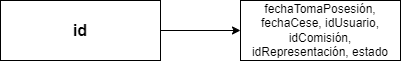
\includegraphics[scale=0.75]{img/diagramas/Datos/FNBC-MiembroComisión.png}
\caption{Tabla MiembroComisión en FNBC}\label{fig:Tabla MiembroComisión en FNBC}   
\end{figure}

 \section{Esquema relacional}\label{sec:esquema-relacional}

\begin{table}[H]
\begin{center}
    \begin{tabular}{|l|p{8cm}|}
    \hline
    Tabla                 &   Atributos          
    \\ \hline
    TipoCentro             &   (\textbf{\underline{id}}, nombre, estado) 
    \\  \hline
    TipoRepresentaciónGobierno          &   (\textbf{\underline{id}}, nombre, estado)
    \\  \hline
    TipoRepresentaciónGeneral             &   (\textbf{\underline{id}}, nombre, estado) 
    \\  \hline
    TipoConvocatoria             &   (\textbf{\underline{id}}, nombre, estado) 
    \\  \hline
    Usuario             &   (\textbf{\underline{id}}, name, email, password, estado) 
    \\  \hline
    Centro             &   (\textbf{\underline{id}}, nombre, dirección, idTipo, estado) 
    \\  \hline
    Junta             &   (\textbf{\underline{id}}, fechaConstitución, fechaDisolución, idCentro, estado) 
    \\  \hline
    Comisión             &    (\textbf{\underline{id}}, nombre, descripción, fechaConstitución, fechaDisolución, idJunta, estado) 
    \\  \hline
    Convocatoria             &    (\textbf{\underline{id}}, lugar, fecha, hora, idTipo, idJun, idCom, estado)
    \\  \hline
    MiembroGobierno             &   (\textbf{\underline{id}}, fechaTomaPosesión, fechaCese, idUsuario, idCentro, idRepresentación, estado) 
    \\  \hline
    MiembroJunta             &   (\textbf{\underline{id}}, fechaTomaPosesión, fechaCese, idUsuario, idJunta, idRepresentación, estado)
    \\  \hline
    MiembroComisión             &   (\textbf{\underline{id}}, fechaTomaPosesión, fechaCese, idUsuario, idComisión, idRepresentación, estado)
    \\  \hline
            \end{tabular}
        \end{center}
    \end{table}



\section{Diagrama relacional}\label{sec:diagrama-relacional}
El diagrama relacional del modelo propuesto se muestra en la figura \ref{fig:Diagrama Relacional}.

\begin{landscape}
\begin{figure}[H]
\centering
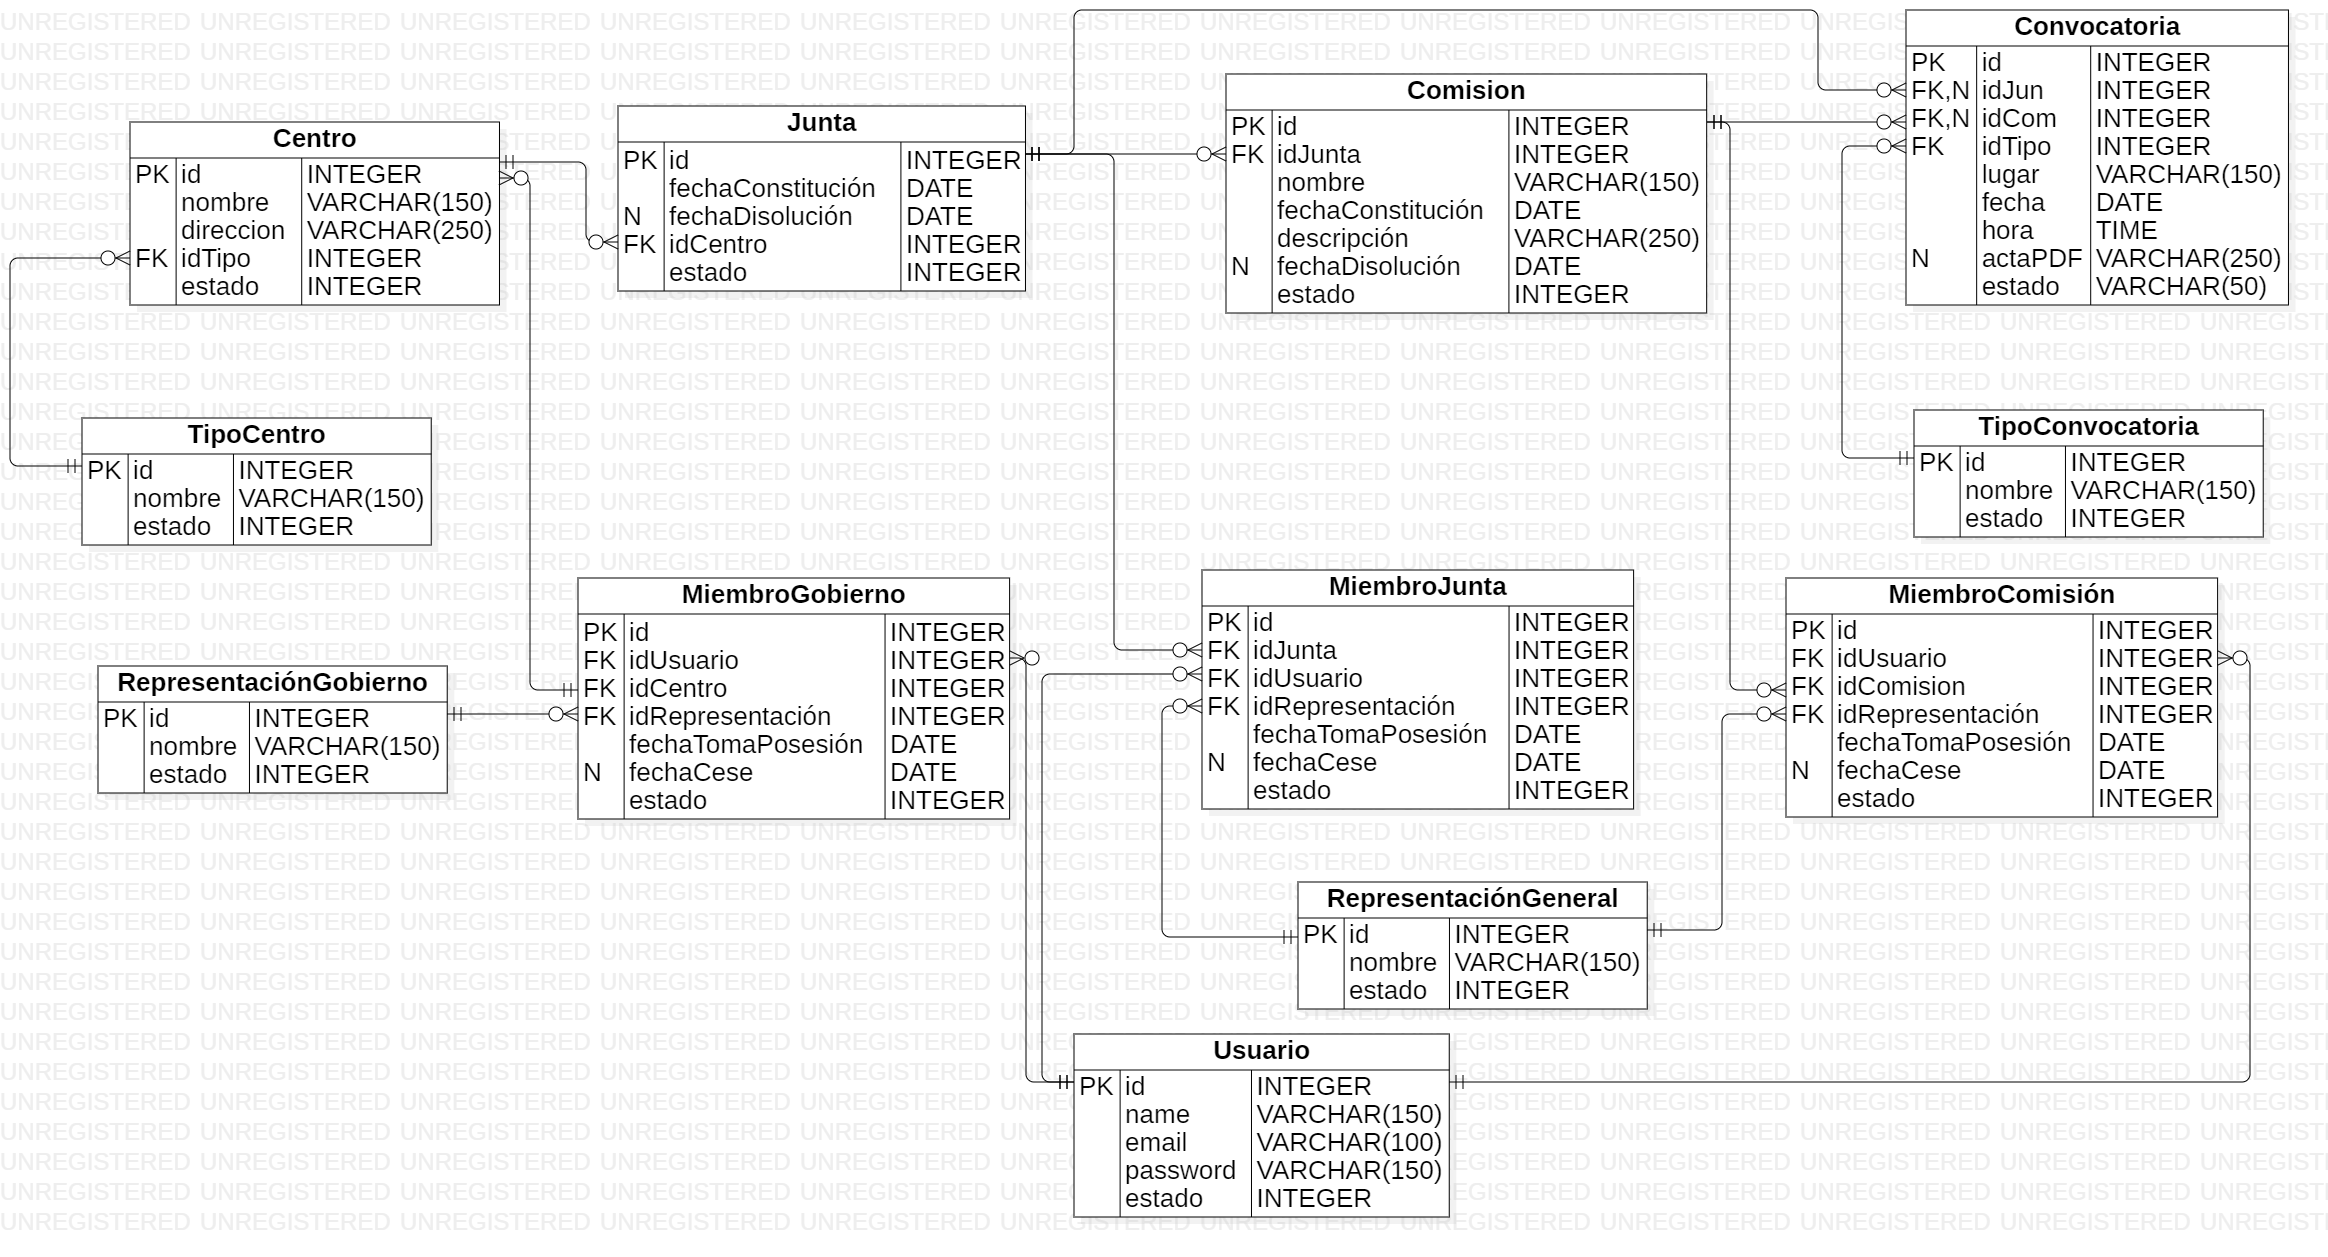
\includegraphics[scale=0.3]{img/diagramas/Datos/Diagrama-relacional.png}
\caption{Diagrama relacional}\label{fig:Diagrama Relacional}   
\end{figure}
\end{landscape}



